\documentclass[12pt,letterpaper]{article}
\usepackage[utf8]{inputenc}
\usepackage[spanish,mexico]{babel}
\usepackage{amsmath}
\usepackage{amsfonts}
\usepackage{amssymb}
\usepackage{amsmath}
\usepackage[lmargin=3cm,rmargin=3cm,tmargin=3cm,bmargin=3cm]{geometry}

\usepackage{hyperref}
\usepackage{graphicx}
\usepackage{float}


\begin{document}

\title{Actividad 3: Interpolar en Python}
\author{Luisa Fernanda Orci Fernandez.}
\date{08 de Febrero del 2016}

\maketitle

\section*{Interpolación}

El punto principal de esta actividad fue el de utilizar la herramienta de python para realizar interpolaciones a funciones dadas, así como gráficarlas.

La interpolación es la obtención de puntos nuevos a partir de un conjunto discreto de puntos. Nos permite aproximar una función complicada con una mas simple. Si se cuenta con una función en la cual resulta "tedioso" su cálculo, si contamos con algunos de sus valores podemos interpolar esta función con una mas sencilla. En general, no obtendremos los mismos valores evaluando en la que obtuvimos y en la original, pero obtenemos resultados muy cercanos a esta.

La interpolación es líneal cuando se toman dos puntos, es cuadrática si utilizamos 3 y así sucesivamente, entre mas grande sea el grado del polinomio que interpola a la función es mejor, ya que se aproxima mas. 

Para realizar esto en Python, utilizamos el comando $SciPyinterpolate$, este nos permite aproximar una función con el uso de puntos aleatorios en el intervalo dado. 

Inicialmente se nos proporcionó un código en el cual se muestra como utilizar este comando; 

\begin{verbatim}
import numpy as np
import matplotlib.pyplot as plt
from scipy.interpolate import interp1d

# Original "data set" --- 21 random numbers between 0 and 1.
x0 = np.linspace(-1,1,21)
y0 = np.random.random(21)

plt.plot(x0, y0, 'o', label='Data')

# Array with points in between those of the data set for interpolation.
x = np.linspace(-1,1,101)

# Available options for interp1d
options = ('linear', 'nearest', 'zero', 'slinear', 'quadratic', 'cubic', 10)

for o in options:
    f = interp1d(x0, y0, kind=o)    # interpolation function
    plt.plot(x, f(x), label=o)      # plot of interpolated data

plt.legend()
plt.show()
\end{verbatim}
Y apartir de el debiamos realizar las siguientes modificaciones:

\begin{itemize}
\item Dados 10 puntos aleatorios entre $x = 0$ y $x = 3$ para la función $f(x) = \sin(2x)$.
\item Dados 20 puntos aleatorios entre $x = -10$ y $x = 10$ para la función $f(x) = \frac{\sin{x}}{x}$.
\item Dados 16 puntos aleatorios entre $x = -3$ y $x = 3$ para la función $f(x) = x^2 \sin(2x)$.
\item Dados 12 puntos aleatorios entre $x = -2$ y $x = 2$ para la función $f(x) = x^3 \sin(3x)$.
\end{itemize}

\newpage

\section{Códigos finales}
A continuación se muestran los códigos modificados junto con su gráfica. 

\subsection{$f(x) = \sin(2x)$}

\begin{verbatim}
import numpy as gatito
import matplotlib.pyplot as plt
from scipy.interpolate import interp1d
from math import sin

x00 = gatito.random.random(10)
x0 = 3*x00

y0 = gatito.sin(2*x0)

plt.plot(x0, y0, 'o', label='Data')

x = gatito.linspace(min(x0), max(x0), 101)

options = ('linear', 'quadratic', 'cubic')

for o in options:
    f = interp1d(x0, y0, kind=o)
    plt.plot(x, f(x), label=o)

plt.legend()
plt.show()
\end{verbatim}
Gráfica:\\
\\
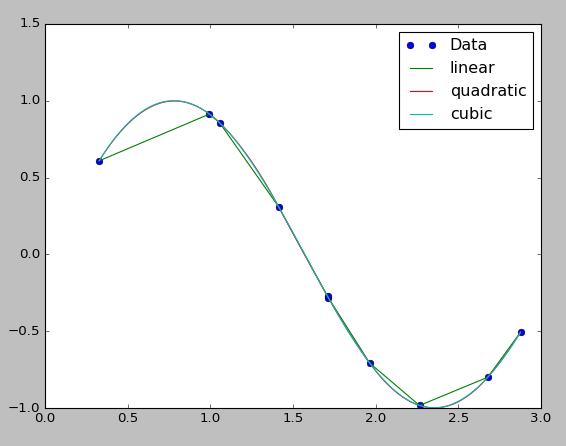
\includegraphics[scale=.5]{grafica1act3.png}

\subsection{$f(x) = \frac{\sin{x}}{x}$}

\begin{verbatim}
import numpy as gatito
import matplotlib.pyplot as plt
from scipy.interpolate import interp1d
from math import sin

x00 = gatito.random.random(20)
x0 = 20*x00-10
y0 = gatito.sin(x0)/x0

plt.plot(x0, y0, 'o', label='Data')

x = gatito.linspace(min(x0), max(x0), 101)

options = ('linear', 'quadratic', 'cubic')

for o in options:
    f = interp1d(x0, y0, kind=o)
    plt.plot(x, f(x), label=o)
plt.legend()
plt.show()

\end{verbatim}

Gráfica:\\
\\
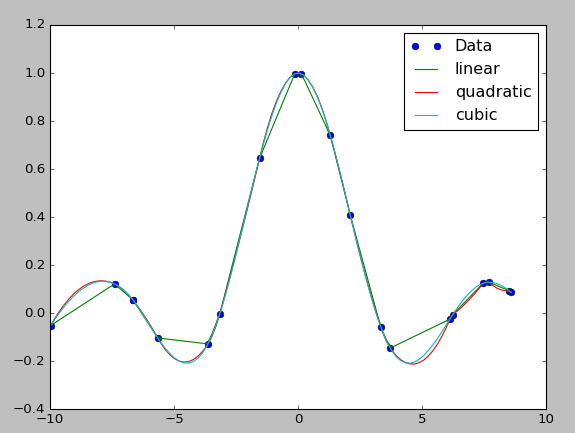
\includegraphics[scale=.5]{grafica2act3.png}

\subsection{$f(x) = x^2 \sin(2x)$}

\begin{verbatim}
import numpy as gatito
import matplotlib.pyplot as plt
from scipy.interpolate import interp1d
from math import sin

x00 = gatito.random.random(16)
x0 = 6*x00-3
y0 = x0**2*gatito.sin(2*x0)

plt.plot(x0, y0, 'o', label='Data')



x= gatito.linspace(min(x0), max(x0), 101)
options = ('linear', 'quadratic', 'cubic')

for o in options: 
    f = interp1d(x0, y0, kind=o)
    plt.plot(x, f(x), label=o)
    
plt.legend()
plt.show()

\end{verbatim}
Gráfica:\\
\\
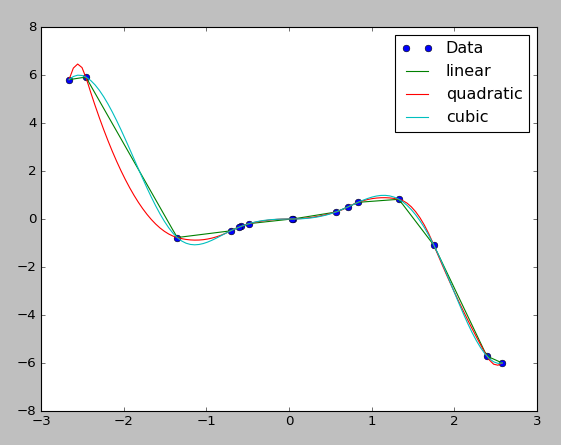
\includegraphics[scale=.5]{grafica3act3.png}

\subsection{$f(x) = x^3 \sin(3x)$}

\begin{verbatim}
import numpy as gatiux
import matplotlib.pyplot as plt
from scipy.interpolate import interp1d
from math import sin

x00 = gatiux.random.random(12)
x0 = 4*x00-2
y0 = x0**3*gatiux.sin(3*x0)

plt.plot(x0, y0, 'o', label='Data')

x = gatiux.linspace(min(x0), max(x0), 101)

options = ('linear', 'quadratic', 'cubic')

for o in options:
    f = interp1d(x0, y0, kind=o)
    plt.plot(x, f(x), label=o)

plt.legend()
plt.show()
\end{verbatim}
Gráfica:\\
\\
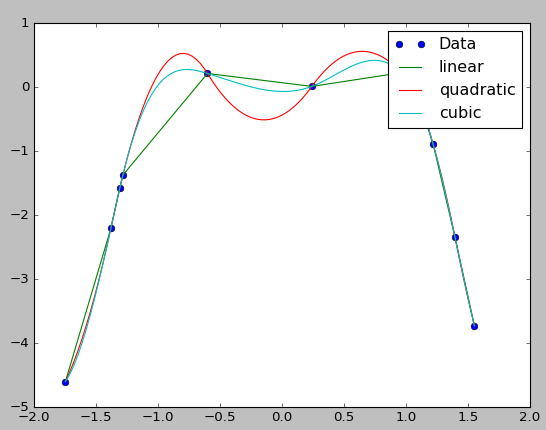
\includegraphics[scale=.5]{grafica4act3.png}

\section*{Conclusiones}

Fue una actividad muy interesante ya que nos ayuda a entender como hacer interpolaciones en Python. 


\begin{thebibliography}{widestlabel}
\bibitem{w} Wikipedia, https://en.wikipedia.org
\bibitem{w} http://computacional1.pbworks.com/w/page/104792695/Actividad\%203\%20\%282016-1\%29
\end{thebibliography}





\end{document}